\chapter{Phase, Polarization, and Unitary Evolution}

This lecture begins with unfinished business and ends with the basic structure of quantum dynamics. We start by returning to photon polarization, because that two-state system is still the cleanest laboratory for the ideas on the board. From there the lecture pauses to ask what state-vectors are actually for, why multiplying a state by an overall phase changes nothing observable, how many parameters are needed to specify the polarization of a photon, and finally what kind of transformations can move states forward in time without disturbing their physical relations. What follows keeps close to that progression. The original lecture is due to Leonard Susskind, and the supporting curation pipeline is credited to LazyingArt LLC and Video2Book.

\section{Polarization Observables Revisited}

The lecture opens by asking for the homework answer: what operator has the circular polarization states as its eigenvectors? Before going on, Susskind quickly reconstructs the three polarization observables that have been developed in the preceding lectures. This is not merely review. He wants the two-state example back on the board before any more formalism is introduced.

For horizontal and vertical polarization we take
\begin{equation}
\hat P_{xy}=
\begin{pmatrix}
1&0\\
0&-1
\end{pmatrix},
\qquad
|x\rangle=
\begin{pmatrix}
1\\
0
\end{pmatrix},
\qquad
|y\rangle=
\begin{pmatrix}
0\\
1
\end{pmatrix}.
\end{equation}
Thus $|x\rangle$ and $|y\rangle$ are eigenvectors of $\hat P_{xy}$ with eigenvalues $+1$ and $-1$.

For linear polarization along an axis making angle $\theta$ with the $x$-direction, the state is written
\begin{equation}
|\theta\rangle=
\begin{pmatrix}
\cos\theta\\
\sin\theta
\end{pmatrix}.
\end{equation}
An orthogonal partner may be chosen as
\begin{equation}
|\theta+\pi/2\rangle=
\begin{pmatrix}
\sin\theta\\
-\cos\theta
\end{pmatrix},
\end{equation}
or with the opposite overall sign. The lecture explicitly remarks that the sign choice does not matter. That is a local comment at first, but by the end of the lecture it becomes a special case of the general irrelevance of overall phase.

The special $45^\circ$ states are therefore
\begin{equation}
|45^\circ,+\rangle=\frac{1}{\sqrt2}
\begin{pmatrix}
1\\
1
\end{pmatrix},
\qquad
|45^\circ,-\rangle=\frac{1}{\sqrt2}
\begin{pmatrix}
1\\
-1
\end{pmatrix},
\end{equation}
and the corresponding observable is
\begin{equation}
\hat P_{45}=
\begin{pmatrix}
0&1\\
1&0
\end{pmatrix}.
\end{equation}

Then comes the genuinely new case, the first place in this story where complex numbers are unavoidable:
\begin{equation}
|C_+\rangle=\frac{1}{\sqrt2}
\begin{pmatrix}
1\\
i
\end{pmatrix},
\qquad
|C_-\rangle=\frac{1}{\sqrt2}
\begin{pmatrix}
1\\
-i
\end{pmatrix}.
\end{equation}
These are again orthogonal, provided we remember the rule that inner products involve complex conjugation. The circular-polarization observable is
\begin{equation}
\hat P_{\mathrm{circ}}=
\begin{pmatrix}
0&-i\\
i&0
\end{pmatrix},
\end{equation}
and one checks directly that
\begin{equation}
\hat P_{\mathrm{circ}}|C_\pm\rangle=\pm |C_\pm\rangle.
\end{equation}

Already the lecture is stressing an operational reading of the mathematics. Orthogonality is not being introduced as a decorative algebraic relation. Two polarization states are orthogonal when they are distinguishable in a single ideal experiment.

\section{What Quantum States Are For}

Now the lecture steps back and asks a broader question: where are we relative to the first discussion of classical mechanics? In the classical setting of a coin, a die, or any finite collection of states, a state was just a point in a set. An observable was merely a numerical label assigned to each point. Time evolution then carried one point to another.

Quantum mechanics has already gone beyond that. The space of states is now a vector space, and observables are operators on that space. But we are not quite ready for dynamics. First we need to say clearly what physically interesting things one does with states once one has them.

There are, in this lecture, two central uses.

First, if the system is in the state $|\psi\rangle$ and we are interested in an observable $\hat K$, we form the expectation value
\begin{equation}
\langle \hat K\rangle_\psi=\langle\psi|\hat K|\psi\rangle.
\end{equation}
This is the quantity we would obtain by preparing the same state over and over and averaging many measurements of $K$.

Second, suppose $|a\rangle$ and $|b\rangle$ are eigenvectors of two different observables:
\begin{equation}
\hat K|a\rangle=\alpha |a\rangle,
\qquad
\hat L|b\rangle=\beta |b\rangle.
\end{equation}
If we prepare the system with a definite value $K=\alpha$ and then measure $L$, the probability to find $L=\beta$ is
\begin{equation}
P(a\to b)=|\langle b|a\rangle|^2
=\langle a|b\rangle\langle b|a\rangle.
\end{equation}
The lecture notes that the same number is obtained if we reverse the order of preparation and measurement. At this level the two great questions are ensemble averages and transition probabilities.

This is the bridge to the phase discussion. If some change in the state-vector does not alter expectation values or transition probabilities, then it has no physical significance.

\section{Overall Phase Has No Physical Meaning}

Before discussing phase, Susskind inserts the normalization rule. Physical state-vectors are taken to be unit vectors:
\begin{equation}
\langle\psi|\psi\rangle=1.
\end{equation}
That fixes the total probability to be one. But it does not yet exhaust the redundancies in the description.

To make the next point precise, the lecture briefly reviews complex numbers. A complex number can be written in rectangular form as $x+iy$ and in polar form as
\begin{equation}
z=re^{i\theta}.
\end{equation}
Its complex conjugate is
\begin{equation}
z^*=re^{-i\theta}.
\end{equation}
A \emph{pure phase} is a complex number of unit modulus, so $r=1$ and
\begin{equation}
z=e^{i\theta},
\qquad
z^*=e^{-i\theta},
\qquad
zz^*=1.
\end{equation}
These are the points on the unit circle in the complex plane.

\begin{figure}[t]
\centering

\includegraphics[width=0.72\textwidth]{lecture_07_figure_02.png}
\caption{Phase-related state vectors and unit-circle sketch from the lecture board.}
\end{figure}

\begin{figure}[t]
\centering
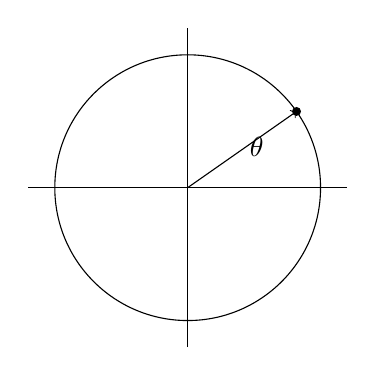
\begin{tikzpicture}[scale=1.35]
\draw (0,0) circle (1.25);
\draw (-1.5,0)--(1.5,0);
\draw (0,-1.5)--(0,1.5);
\draw[->] (0,0)--(35:1.25);
\fill (35:1.25) circle (1.2pt);
\node at (0.65,0.38) {$\theta$};
\end{tikzpicture}
\caption{Clean reconstruction of the phase-circle picture used in the lecture.}
\end{figure}

On the board this geometric picture is paired with a comparison of two vectors,
\begin{equation}
|A\rangle,
\qquad
e^{i\theta}|A\rangle.
\end{equation}
Mathematically they are different vectors. The second is the first multiplied by a complex number. But physically the lecture insists that they describe the same state. The point is not asserted as a slogan; it is checked against the two things states are used for.

Let
\begin{equation}
|\psi'\rangle=e^{i\chi}|\psi\rangle.
\end{equation}
Then the corresponding bra is
\begin{equation}
\langle\psi'|=e^{-i\chi}\langle\psi|.
\end{equation}
So the expectation value of any observable is unchanged:
\begin{align}
\langle\psi'|\hat K|\psi'\rangle
&=
e^{-i\chi}\langle\psi|\hat K\,e^{i\chi}|\psi\rangle \\
&=
e^{-i\chi}e^{i\chi}\langle\psi|\hat K|\psi\rangle \\
&=
\langle\psi|\hat K|\psi\rangle.
\end{align}
The phase cancels because it is only an ordinary number.

The same happens for transition probabilities. If, for example, we replace $|b\rangle$ by $e^{i\chi}|b\rangle$, then
\begin{align}
|\langle e^{i\chi}b|a\rangle|^2
&=
\langle a|e^{i\chi}b\rangle \langle e^{i\chi}b|a\rangle \\
&=
e^{i\chi}e^{-i\chi}\langle a|b\rangle\langle b|a\rangle \\
&=
|\langle b|a\rangle|^2.
\end{align}
Again the phase disappears.

This is why the lecture is willing to say that there is no physical significance to the overall phase of the wave function. The physical state is not a single vector but an equivalence class under multiplication by a pure phase.

A simple example is already available:
\begin{equation}
|y\rangle=
\begin{pmatrix}
0\\
1
\end{pmatrix},
\qquad
-|y\rangle=
\begin{pmatrix}
0\\
-1
\end{pmatrix}.
\end{equation}
The second vector is $e^{i\pi}|y\rangle$. It is not equal to the first one, but it has the same physical significance.

Likewise
\begin{equation}
\frac{1}{\sqrt2}
\begin{pmatrix}
1\\
i
\end{pmatrix}
\qquad\text{and}\qquad
\frac{1}{\sqrt2}
\begin{pmatrix}
i\\
-1
\end{pmatrix}
\end{equation}
differ by the phase $i=e^{i\pi/2}$ and therefore represent the same circular polarization state.

\subsection{Question \& Answer}

If $|\psi\rangle$ and $e^{i\theta}|\psi\rangle$ are mathematically different vectors, why are they physically the same?

Because all the physical questions under discussion in this lecture are built from bra-ket sandwiches and squared overlaps. In every such expression an overall phase meets its complex conjugate and cancels. So the distinction is real mathematically but empty physically. The lecture briefly experiments with an ad hoc symbol for this equivalence; in the notes it is safer simply to say that the two vectors have the same physical significance.

\section{Counting the Parameters of Photon Polarization}

At this point phase indifference begins to do real work. It is not merely that phase happens to cancel from a few formulas; we may now divide by that redundancy and count the truly physical parameters of photon polarization.

Start from the most general two-component state,
\begin{equation}
|\psi\rangle=
\begin{pmatrix}
\alpha\\
\beta
\end{pmatrix},
\end{equation}
with $\alpha$ and $\beta$ complex. That is four real parameters. Normalization imposes one condition,
\begin{equation}
\alpha^*\alpha+\beta^*\beta=1,
\end{equation}
so we are left with three.

Now use the fact that overall phase carries no physical information. By multiplying the whole state by a suitable phase, we can always choose the upper component to be real. Call it $a\in\mathbb R$. Then normalization becomes
\begin{equation}
a^2+\beta^*\beta=1.
\end{equation}
Hence
\begin{equation}
\beta^*\beta=1-a^2,
\end{equation}
and so the lower component may be written as
\begin{equation}
\beta=\sqrt{1-a^2}\,e^{i\phi}.
\end{equation}
Here the lecture repairs the notation: the phase is now renamed $\phi$ so that $\theta$ may continue to denote a linear-polarization angle.

Thus the general physical polarization state may be written in the gauge-fixed form
\begin{equation}
|\psi\rangle=
\begin{pmatrix}
a\\
\sqrt{1-a^2}\,e^{i\phi}
\end{pmatrix}.
\end{equation}
There are exactly two real parameters left: the real number $a$ and the phase angle $\phi$.

The important point is not merely the counting itself. The lecture immediately asks what those two parameters mean physically. That question is what carries us from state-vector coordinates back to the actual geometry of electromagnetic waves.

\section{From State Vectors to Elliptical Polarization Geometry}

The lecture now shifts language. Up to this point we have been talking in the coordinates of a two-dimensional complex vector space. But photon polarization is not only an algebraic construction. It is also the motion of the electric field of an electromagnetic wave in the plane transverse to propagation.

A plane-polarized wave has its electric field along a single axis. If the wave is moving into the board, the direction of that axis is one parameter. So purely linear polarization gives only a one-parameter family.

If we combine two linear polarizations whose components are in phase, the result is still plane polarization, just along a different axis. But if the two components are out of phase, the electric field need no longer move on a line. It may move on a circle, and more generally on an ellipse.

The lecture gives simple examples. If
\begin{equation}
E_x=\cos(x-ct),
\qquad
E_y=\sin(x-ct),
\end{equation}
then at fixed $x$, say $x=0$, the tip of the electric field moves on a circle. That is circular polarization. If instead we take
\begin{equation}
E_x=\cos(x-ct),
\qquad
E_y=\frac12\sin(x-ct),
\end{equation}
then at fixed $x$ the field traces an ellipse, in this case with major axis along the $x$-direction.

So the geometry carries two physical parameters:
\begin{enumerate}
\item the direction of the major axis,
\item the shape of the ellipse, described in the lecture by its eccentricity or aspect-ratio parameter.
\end{enumerate}
This matches the algebraic count perfectly. The two real parameters in the state-vector are not literally the angle and the eccentricity, but there is a one-to-one correspondence: some functions of them are the angle of the long axis and the shape parameter of the ellipse.

The lecture also pauses over the limiting cases. When the ellipse collapses to a line, we recover plane polarization. When it becomes a circle, the major axis ceases to matter because no axis is distinguished.

\subsection{Question \& Answer}

Where did clockwise versus counterclockwise polarization go if there are only two real parameters?

The lecture answers this in a deliberately geometric way. Start from circular polarization and squeeze the circle into an ellipse. Continue squeezing until the ellipse collapses to a line. If one keeps going past that point, the upper and lower branches exchange roles and the sense of rotation reverses. So the single shape parameter is extended through zero and into negative values. In that lecture language, one may think of the second sense of rotation as being encoded by \emph{negative eccentricity}. It is a heuristic description, but it is exactly the one used to show that two real parameters are enough.

\section{Overlap With Linear Polarization and the Major Axis}

The lecture now asks a more practical question. Suppose a photon is in a general elliptically polarized state. How do we recover the direction of its major axis from measurement probabilities?

We compare the elliptic state with the linearly polarized state at analyzer angle $\theta$:
\begin{equation}
|\theta\rangle=
\begin{pmatrix}
\cos\theta\\
\sin\theta
\end{pmatrix},
\qquad
|\psi\rangle=
\begin{pmatrix}
a\\
\sqrt{1-a^2}\,e^{i\phi}
\end{pmatrix}.
\end{equation}
Operationally this means: put a linear polarizer at angle $\theta$ in the path of the photon and ask for the probability that the photon passes through.

\begin{figure}[t]
\centering

\includegraphics[width=0.82\textwidth]{lecture_07_figure_03.png}
\caption{State-vector overlap and geometric sketches as laid out across the lecture boards.}
\end{figure}

On the board the bra-ket order is partly obscured, and in the spoken derivation Susskind corrects himself by remembering that one factor must be complex conjugated. In a cleaned form consistent with that correction, we may record the overlap as
\begin{equation}
\langle\psi|\theta\rangle
=
a\cos\theta+\sqrt{1-a^2}\,e^{-i\phi}\sin\theta.
\end{equation}
If one writes the overlap in the opposite order, the phase is conjugated accordingly; the probability is the same either way.

\begin{figure}[t]
\centering
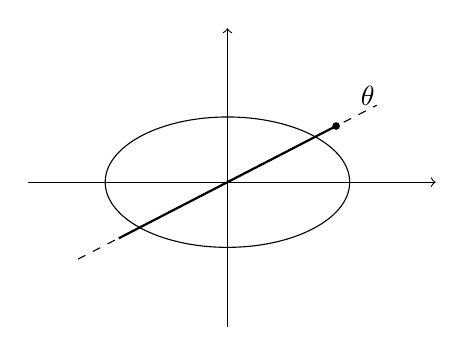
\begin{tikzpicture}[scale=1.15]
\draw[->] (-2.2,0)--(2.3,0);
\draw[->] (0,-1.6)--(0,1.7);
\draw (0,0) ellipse (1.35 and 0.72);
\draw[dashed] (-1.65,-0.85)--(1.65,0.85);
\draw[thick] (-1.2,-0.62)--(1.2,0.62);
\fill (1.2,0.62) circle (1.2pt);
\node at (1.55,0.95) {$\theta$};
\end{tikzpicture}
\caption{Conservative reconstruction of the geometric guide used in the lecture: vary the analyzer direction until the overlap with the elliptic state is maximal.}
\end{figure}

The transmission probability is therefore
\begin{equation}
P_\theta(\psi)=|\langle\psi|\theta\rangle|^2.
\end{equation}
Here the lecture deliberately stops short of a fully polished computation. Susskind does not expand the modulus squared on the board; instead he assigns that algebra as homework. But the next step is perfectly clear. We keep $\phi$ fixed, regard $\theta$ as the variable analyzer angle, and maximize:
\begin{equation}
\frac{d}{d\theta}P_\theta(\psi)=0.
\end{equation}
The value of $\theta$ that maximizes $P_\theta(\psi)$ gives the direction of the major axis.

The lecture says much less about the ellipse parameter itself. The suggestion is qualitative rather than finished: compare the probabilities for transmission along the major and minor directions, and their difference measures the asymmetry of the ellipse. Since the lecture does not derive a closed formula here, the notes should not invent one.

\section{Time Evolution, Hermitian Operators, and the Unitary Pivot}

Up to this point the states have been standing still on the board. The next step is the big one: how do quantum states change with time? The lecture begins from the classical analogy and then formalizes the quantum answer.

\subsection{Relations Between States}

In classical mechanics with finitely many states, time evolution is essentially a permutation of those states. Different initial states remain different. If two distinct states both evolved into the same final state, information about the initial condition would be lost.

Quantum mechanics has a richer notion of relation between states. Two normalized states may be the same, orthogonal, or somewhere in between. The operational example remains polarization. A vertically polarized photon does not pass a horizontal polarizer, so
\begin{equation}
\langle y|x\rangle=0
\end{equation}
expresses a definite physical distinction. By contrast, for normalized states,
\begin{equation}
\langle B|A\rangle=1
\end{equation}
means that the two states are the same state, up to the phase distinction that we have already agreed to ignore physically.

So the lecture identifies the basic relation between states with the inner product. Zero means orthogonal, one means identical normalized states, and intermediate values measure partial overlap and therefore partial distinguishability.

The quantum analog of classical distinction-preservation is then that inner products remain fixed in time. If
\begin{equation}
|A\rangle\to |A'\rangle,
\qquad
|B\rangle\to |B'\rangle,
\end{equation}
then
\begin{equation}
\langle B'|A'\rangle=\langle B|A\rangle.
\end{equation}
In particular, states that start orthogonal stay orthogonal.

This is presented in the lecture as a physical principle rather than a theorem derived from something more primitive. It is taken as an observed fact, one that fits together with deeper conservation ideas and, above all, with the requirement that quantum time evolution not destroy distinctions between states.

\subsection{Hermitian Conjugation And Hermitian Operators}

To implement that idea we need more mathematics. The lecture now reviews linear operators with some care.

Let $L$ be a linear operator defined by its action on kets. If
\begin{equation}
L|A\rangle=|C\rangle,
\end{equation}
then we also want a consistent way to let such an operator appear in bra-ket sandwiches. In a complete orthonormal basis,
\begin{equation}
\sum_n |n\rangle\langle n|=I.
\end{equation}
This allows us to define matrix elements
\begin{equation}
\langle B|L|A\rangle,
\end{equation}
which the lecture emphasizes can be interpreted either by first acting with $L$ on the ket and then taking the inner product with $\langle B|$, or by using the corresponding action on bras and then pairing with $|A\rangle$.

From there the lecture introduces the Hermitian conjugate. Cleanly stated, the rule is
\begin{equation}
\langle n|L^\dagger|m\rangle=\langle m|L|n\rangle^*,
\end{equation}
or in matrix notation,
\begin{equation}
(L^\dagger)_{nm}=L_{mn}^*.
\end{equation}
So Hermitian conjugation is obtained by transposing and then complex conjugating.

An operator is Hermitian when
\begin{equation}
L=L^\dagger.
\end{equation}
This immediately implies two componentwise facts:
\begin{equation}
L_{ii}=L_{ii}^*,
\end{equation}
so the diagonal entries are real, and
\begin{equation}
L_{ij}=(L_{ji})^*,
\end{equation}
so entries reflected across the diagonal are complex conjugates of one another.

The lecture then checks the polarization observables one by one:
\begin{equation}
\hat P_{xy}=
\begin{pmatrix}
1&0\\
0&-1
\end{pmatrix},
\qquad
\hat P_{45}=
\begin{pmatrix}
0&1\\
1&0
\end{pmatrix},
\qquad
\hat P_{\mathrm{circ}}=
\begin{pmatrix}
0&-i\\
i&0
\end{pmatrix}.
\end{equation}
All three are plainly Hermitian.

At this point the lecture recalls the standard physical content of Hermitian operators. Their expectation values are real, their eigenvalues are real, and their eigenvectors form a complete orthonormal basis. That is why observables are represented by Hermitian operators.

The lecture also remarks that real quantum systems are usually infinite-dimensional. The finite-dimensional matrix language is being used because it displays the structure clearly, and because in practice even infinite-dimensional problems are often approximated by very large matrices.

\subsection{Unitary Operators}

But Hermitian operators are not the transformations we need for time evolution. Observables tell us what can be measured. Time evolution requires operators that preserve relations between states.

Let $U$ be such a transformation:
\begin{equation}
U|A\rangle=|A'\rangle,
\qquad
U|B\rangle=|B'\rangle.
\end{equation}
Then the corresponding bras transform with $U^\dagger$:
\begin{equation}
\langle A'|=\langle A|U^\dagger,
\qquad
\langle B'|=\langle B|U^\dagger.
\end{equation}
Now impose the physical requirement that the inner product be preserved:
\begin{align}
\langle B'|A'\rangle
&=
\langle B|U^\dagger U|A\rangle \\
&=
\langle B|A\rangle.
\end{align}
If this is true for every pair of states $|A\rangle$ and $|B\rangle$, then the operator between them must be the identity:
\begin{equation}
U^\dagger U=I.
\end{equation}
Equivalently,
\begin{equation}
U^\dagger=U^{-1}.
\end{equation}
That is the defining property of a unitary operator.

The lecture insists on the right reading of this equation. A unitary operator is not itself the identity. It can move vectors around the state space, rotate polarization directions, or represent time evolution. What makes it unitary is that it moves vectors around without altering the inner products that encode physical relations and probabilities.

This is the closing message of the lecture. Systems change with time by unitary transformations. The detailed properties of unitary eigenvalues are left for the next lecture, together with the introduction of Hamiltonians. Here we stop at the threshold: the correct mathematical form of quantum evolution has now been identified.

\section{Summary}

The lecture begins by tying up the polarization story and ends by opening the door to quantum dynamics. Along the way we see three ideas lock together. First, the physically meaningful uses of a state-vector are expectation values and transition probabilities. Second, both are insensitive to an overall phase, so the physical state is represented by a normalized vector only up to multiplication by a pure phase. Third, once the relation between states is recognized as the inner product, the natural transformations of state space are those that preserve that inner product, namely the unitary operators. Photon polarization remains the anchor throughout, but the lesson is much broader: the geometry of state space, not just the list of possible outcomes, is what controls the way quantum mechanics evolves in time.